\documentclass[conference]{IEEEtran}
\IEEEoverridecommandlockouts

% --- Packages (safe for IEEEtran) ---
\usepackage{cite}
\usepackage{amsmath,amssymb}
\usepackage{graphicx}
\usepackage{booktabs}
\usepackage{multirow}
\usepackage{url}
\usepackage{array}
\usepackage{listings}
\usepackage{tikz}
\usetikzlibrary{arrows.meta,positioning,fit,calc}
\usepackage{stfloats} % Helps with figure* placement

% --- Listings style (compact) ---
\lstset{
  basicstyle=\ttfamily\footnotesize,
  columns=fullflexible,
  breaklines=true,
  frame=single,
  xleftmargin=1em,
  xrightmargin=1em,
  framesep=1em,
  aboveskip=0.6em,
  belowskip=0.6em,
  abovecaptionskip=1em,
  captionpos=b
}

\begin{document}

\title{Comparing LLMs in Forming Predictions and Analyses based on Spotify Audio Features}

\author{
\IEEEauthorblockN{Shunyao Mao \hspace{0.6em} Connor Jin \hspace{0.6em} Yunxi He}
\IEEEauthorblockA{\textit{ELEC 220, Department of Electrical and Computer Engineering}\\
\textit{Rice University, Houston, TX, USA}\\
sm310@rice.edu \hspace{0.6em} cj80@rice.edu \hspace{0.6em} yh181@rice.edu}
}

\maketitle

\begin{abstract}
Large language models (LLMs) are increasingly used as natural-language interfaces to structured datasets, but their reliability on data-grounded tabular tasks remains uncertain. Following our midterm plan, we benchmark three representative LLM families---GPT, Gemini, and Claude---on a Spotify audio-features dataset. We evaluate (i) popularity-bucket classification from numeric audio features with \emph{numeric justifications} constrained to cite real fields and compare to dataset medians, and (ii) text-to-SQL question answering over a fixed SQLite schema. Beyond accuracy, we quantify explanation quality with a 0--5 rubric emphasizing data grounding, specificity, and non-hallucination. We also include a tabular ML baseline (e.g., XGBoost) to contextualize performance and to enable an interpretability cross-check between model rationales and feature-importance rankings.
\end{abstract}

\begin{IEEEkeywords}
large language models, tabular data, music information retrieval, Spotify audio features, text-to-SQL, interpretability, benchmarking
\end{IEEEkeywords}

\section{Introduction}
Music-streaming platforms and research communities have long relied on structured datasets of songs and artists, containing both human-curated data and automatically extracted audio features such as tempo, energy, and valence. With the rapid adoption of large language models (LLMs), analysts can attempt to use such interfaces for exploring and modeling these datasets without writing traditional code.   

However, despite impressive general capabilities, the dependability of LLMs in specialized, data-grounded music tasks is unclear. It's important to understand their textual explanations grounded in evidence and proper analysis, or whether they simply generate relevant keywords. Addressing these questions requires quantitative evaluation.  

This project benchmarks three representative LLMs—GPT, Gemini, and Claude—on realistic music-analytics tasks using Spotify’s publicly available audio features. Our goals are to measure model accuracy and to produce a reproducible evaluation suite that informs both research and practical applications in music intelligence.   

This topic was chosen because of the team’s shared interest in music and AI, and because the results could directly inform research and product decisions. This project blends our everyday background in listening to music with current interest in modern computing and trustworthy AI. The deliverable informs real music-analytics use cases (playlist curation, catalog QA, research) and provides hands-on experience with rigorous LLM evaluation.
% --- FIGURE MOVED HERE FOR FORMATTING ---
% Placing figure* here allows it to float to the top of Page 2 correctly.
\begin{figure*}[t]
\centering
\resizebox{\textwidth}{!}{%
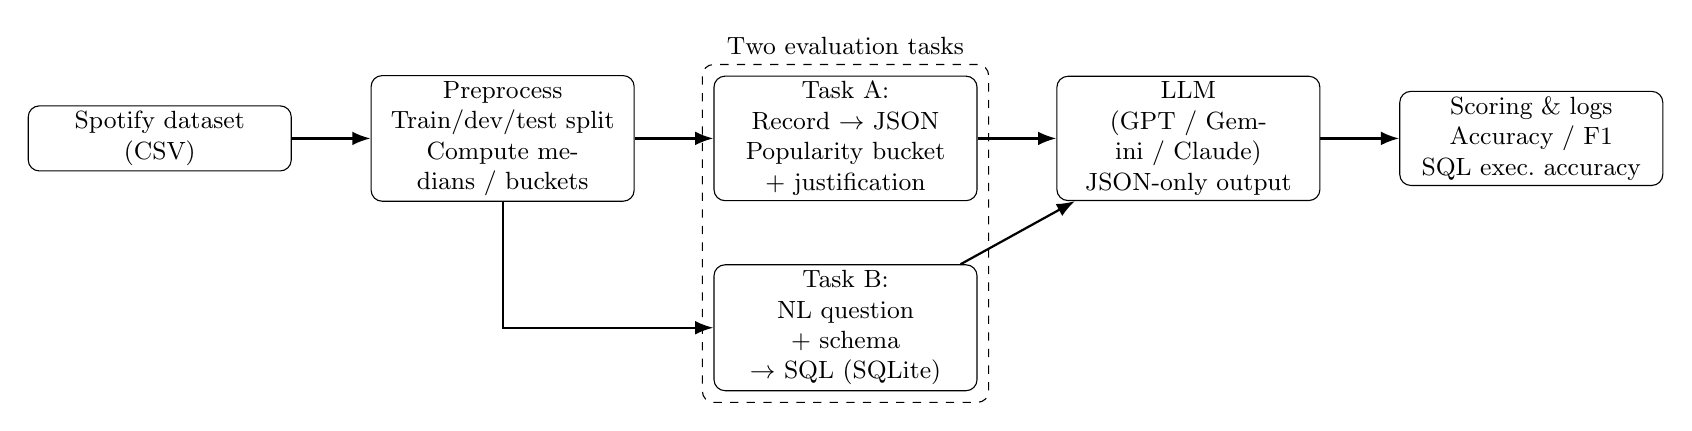
\begin{tikzpicture}[
  font=\small,
  node/.style={
    draw,
    rounded corners,
    align=center,
    minimum height=8mm,
    inner sep=2pt,
    text width=3.2cm
  },
  arrow/.style={-Latex, thick}
]

\node[node] (data) {Spotify dataset\\(CSV)};
\node[node, right=10mm of data] (prep) {Preprocess\\Train/dev/test split\\Compute medians / buckets};
\node[node, right=10mm of prep] (taskA) {Task A:\\Record $\rightarrow$ JSON\\Popularity bucket\\+ justification};
\node[node, below=8mm of taskA] (taskB) {Task B:\\NL question + schema\\$\rightarrow$ SQL (SQLite)};
\node[node, right=10mm of taskA] (llm) {LLM\\(GPT / Gemini / Claude)\\JSON-only output};
\node[node, right=10mm of llm] (score) {Scoring \& logs\\Accuracy / F1\\SQL exec.\ accuracy\\};

\draw[arrow] (data) -- (prep);
\draw[arrow] (prep) -- (taskA);
\draw[arrow] (prep) |- (taskB.west);
\draw[arrow] (taskA) -- (llm);
\draw[arrow] (taskB) -- (llm);
\draw[arrow] (llm) -- (score);

\node[
  draw,
  dashed,
  rounded corners,
  fit=(taskA)(taskB),
  inner sep=4pt,
  label={[font=\small]above:Two evaluation tasks}
] {};

\end{tikzpicture}%
}
\caption{End-to-end evaluation pipeline used in this project.}
\label{fig:pipeline}
\end{figure*}
% ----------------------------------------

\subsection{Contributions}
\begin{itemize}
\item A reproducible evaluation harness for LLMs on (A) popularity-bucket classification with numeric justifications and (B) text-to-SQL over a Spotify schema, using JSON-only outputs.
\item An explanation-quality rubric and interpretability cross-check comparing cited evidence to a tabular baseline's feature-importance ranking.
\end{itemize}

\section{Methodology}
\subsection{Dataset: Spotify Audio Features (Kaggle)}
We will use a Kaggle variant of the Spotify audio-features dataset containing track-level metadata and numeric descriptors retrieved from the Spotify API. Typical fields include track, artist, and album identifiers, release year, popularity (0–100), and audio features such as danceability, energy, valence, tempo (BPM), key, mode, acousticness, instrumentalness, liveness, speechiness, and loudness. Some variants also include artist-level genres.\footnote{Example dataset landing page on Kaggle; we will respect the dataset license and course policies.}

\subsubsection*{Label Engineering}
Our main supervised label is a {\it popularity bucket}: we compute tertiles on the training split and assign LOW/MID/HIGH categories. This balances classes and stabilizes popularity, which can vary over time. If artist genres are present, we will define a coarse genre family (Pop, Rock, Hip-Hop, Dance/Electronic, Other) for an auxiliary classification task.

\subsubsection*{Why This Dataset}
The dataset offers clean tabular structure, well-known numeric features, and large scale—ideal for testing LLM reasoning over structured data and for requiring explanations grounded in numeric evidence.

\subsection{Feature definitions and ranges}
Table~\ref{tab:features} documents the core numeric fields. This table makes the report self-contained and makes ``precise illustrations'' possible without hand-wavy descriptions.

\begin{table}[t]
\centering
\caption{Core Spotify audio features used in Task A. Ranges reflect Spotify API conventions.}
\label{tab:features}
\begin{tabular}{p{2.2cm}p{4.9cm}}
\toprule
\textbf{Feature} & \textbf{Meaning (range)} \\
\midrule
danceability & Suitability for dancing (0--1) \\
energy & Intensity/activ. (0--1) \\
valence & Positiveness (0--1) \\
tempo & Tempo in BPM (approx.\ 0--250+) \\
loudness & Overall loudness (dB, typically $[-60,0]$) \\
acousticness & Acoustic probability (0--1) \\
instrumentalness & Instrumental probability (0--1) \\
liveness & Live-audience probability (0--1) \\
speechiness & Spoken-word probability (0--1) \\
mode, key & Tonal mode (0/1) and pitch class (0--11) \\
year & Release year (integer) \\
\bottomrule
\end{tabular}
\end{table}

\subsection{Label engineering: popularity buckets}
Our primary supervised target is a \emph{popularity bucket}. We define three popularity buckets using fixed ranges: 0–33 (LOW), 34–67 (MID), and 68–100 (HIGH). This reduces sensitivity to exact popularity values and yields approximately balanced classes.

\subsection{Splits and leakage control}
We use artist-level splitting when stable artist IDs exist, to reduce leakage from seeing the same artist in train and test. If only string names exist, we deduplicate by \texttt{(artist, track\_name)} and apply a stratified track-level split. We report the random seed and any filtering in the reproducibility checklist (Table~\ref{tab:repro}).

\section{Tasks}
Figure~\ref{fig:pipeline} shows the end-to-end pipeline used for both tasks. It is drawn directly in \LaTeX{} (TikZ).
\subsection{Task A: Popularity classification with numeric justification}
\textbf{Input:} a JSON record containing numeric features and minimal metadata.\\
\textbf{Output:} a popularity bucket in \{\texttt{LOW, MID, HIGH}\}, a numerical popularity value, and a one-sentence justification that cites at least two numeric fields and compares to dataset medians.

\subsection{Task B: Text-to-SQL question answering}
\textbf{Input:} a natural-language question plus a schema snippet.\\
\textbf{Output:} a JSON wrapper containing an SQLite-compatible SQL query.\\
\textbf{Evaluation:} exact-match (after canonicalization) and \emph{execution accuracy} by running the query on a frozen database and comparing answers to gold.

\subsection{Gold SQL question set design}
We build a gold set of questions covering: (i) simple filters (e.g., ``tracks after 2015 with energy $>$ 0.8''), (ii) aggregations (AVG tempo by year), (iii) top-$k$ ranking (highest danceability), and (iv) grouped comparisons (mean popularity by key/mode). Each question is paired with a canonical SQL query and a deterministic answer extracted from the frozen SQLite DB.

\section{Models and Prompts}
\subsection{Model settings}
We evaluate three LLM families: GPT, Gemini, and Claude, using each provider's stable API model available during the project window. All versions used are the default, publicly accessible ones. We standardize decoding settings across models (temperature, top-$p$, max tokens) and enforce JSON-only outputs for automatic parsing.

\subsection{Risks and Mitigations}
\begin{itemize}
  \item \emph{Sparse or noisy labels:} choose a dataset with reliable labels; use macro-F1.
  \item \emph{Lyrics licensing:} prefer metadata-only tasks or short fair-use snippets.
  \item \emph{LLM rate limits/cost:} cap examples with stratified sampling; cache responses.
  \item \emph{Text-to-SQL brittleness:} restrict SQL surface; provide schema-aware prompts.
\end{itemize}


\subsection{Prompt templates}
We use a schema-aware prompt scaffold. For Task A, we require decisions to be based only on provided fields and require citing at least two numeric features and comparing to dataset medians. For Task B, we provide the table schema with given variables and restrict SQL to listed columns and SQLite-compatible syntax.

Each prompt includes precise information on the data provided. Due to model constraints, the JSON file provided only included subsets of the full Kaggle dataset, with dataset medians provided explicitly in the prompt. Below are the exact prompts we provided to all three LLMs, along with example outputs.

\begin{lstlisting}[caption={Task A prompt},label={lst:promptA}]
We are given a Spotify track record as JSON with fields: {danceability, energy, valence, tempo, loudness, acousticness, instrumentalness, liveness, speechiness, mode1}. Classify POPULARITY_BUCKET as one of {LOW, MID, HIGH}. Provide numerical popularity prediction from 1-100, with 1-33 LOW, 33-67 MID, 68-100 HIGH, . Rules: (1) Base decision only on the provided fields. (2) Cite at least 2 numeric features from JSON. (3) Compare against dataset medians provided below. Return as a JSON only with all songs: {"track_id", "abcd1234", "track_name":, "bucket":"LOW|MID|HIGH","prob":0.0-1.0, "popularity: 1-100", "justification":"<one sentence citing features>", "evidence":{"energy":0.xx,"tempo_bpm":nnn,...}}
MEDIANS:
duration_ms: 212906.0
danceability: 0.58
energy: 0.685
key: 5.0
loudness: -7.004
mode: 1.0
speechiness: 0.0489
acousticness: 0.169
instrumentalness: 4.16e-05
liveness: 0.132
valence: 0.464
tempo: 122.017
time_signature: 4.0
\end{lstlisting}

\begin{lstlisting}[caption={Task A example LLM output},label={lst:promptA}]
[
  {
    "track_id": "6KwkVtXm8OUp2XffN5k7lY",
    "track_name": "No Other Name",
    "bucket": "HIGH",
    "prob": 0.66,
    "popularity": 70,
    "justification": "Energy (0.598) and danceability (0.369) relative to medians (0.685, 0.58) indicate this popularity level.",
    "evidence": {
      "energy": 0.598,
      ...
    }
  },
  {
    "track_id": "2dp5I5MJ8bQQHDoFaNRFtX",
    "track_name": "Failed Organum",
    "bucket": "HIGH",
    "prob": 0.66,
    "popularity": 70,
    "justification": "Energy (0.997) and danceability (0.171) relative to medians (0.685, 0.58) indicate this popularity level.",
    "evidence": {
      "energy": 0.997,
        ...
    }
  },
  ...
]
\end{lstlisting}


\vspace{3ex}
\begin{lstlisting}[caption={Task B Prompt}, label={lst:promptB}]
You are an expert SQL assistant specialized in SQLite.
Your task is to translate natural language questions into valid SQLite queries based on the data structure found in the "song_dataset.json" file.

#DATABASE SCHEMA
Table Name: song_dataset
(Note: Treat the JSON file "song_dataset.json" as a SQL table named 'song_dataset' with the following columns)
Columns:
track_id (text), artists (text), album_name (text), track_name (text), popularity (integer, 0-100), duration_ms (integer), explicit (boolean), danceability (float, 0.0-1.0), energy (float, 0.0-1.0), key (integer, 0-11), loudness (float), mode (integer, 0 or 1), speechiness (float), acousticness (float), instrumentalness (float), liveness (float), valence (float, 0.0-1.0), tempo (float), time_signature (integer), track_genre (text)

### RULES
1. Return ONLY a single valid JSON list (array).
2. Do not include markdown formatting (like ```json), explanations, or extra text. Just the raw JSON.
3. Use only the columns listed in the DATABASE SCHEMA which correspond to the keys in "song_dataset.json".
4. Ensure the SQL is compatible with SQLite.
5. All queries must target the table name 'song_dataset'.
6. Use data from "question_list.json". The "group", "id", and "question" categories should derive their data from this category.
7. Output the JSON list into a file titled "results.json"

### OUTPUT FORMAT
[
  {"id": 1, "group": 1, "question": "Question text here", "sql": "SELECT ... FROM song_dataset WHERE ..."},
  {"id": 2, "group": 1, "question": "Question text here", "sql": "SELECT ... FROM song_dataset WHERE ..."}
]
\end{lstlisting}

\begin{lstlisting}[caption={Task B Example Output}, label={lst:promptB}]
[
  {"id": 1, "group": 1, "question": "Find all tracks with energy greater than 0.8.", "sql": "SELECT * FROM song_dataset WHERE energy > 0.8;"},
  {"id": 2, "group": 1, "question": "List all songs with a danceability score below 0.5 and a tempo above 140 BPM.", "sql": "SELECT * FROM song_dataset WHERE danceability < 0.5 AND tempo > 140;"},
  ...
]
\end{lstlisting}


\subsection{Baselines}
We include:
\begin{itemize}
\item \textbf{Majority-class} baseline for popularity buckets.
\item \textbf{Tabular ML baseline} (e.g., XGBoost or logistic regression) trained on numeric features. This baseline provides contextual performance and supplies feature-importance signals for interpretability checks.
\end{itemize}

\section{Metrics}
\subsection{Classification metrics}
For popularity buckets, we report accuracy and macro-F1. For text-to-SQL, we report exact-match SQL (after normalization) and execution accuracy on the frozen database. Execution accuracy is prioritized because many semantically equivalent SQL strings differ in formatting.

\subsection{Explanation-quality rubric (0--5)}
Each justification is scored using a 0--5 rubric:
\begin{enumerate}
\item \textbf{Data-groundedness} (0--2): cites real numeric fields present in the input.
\item \textbf{Specificity} (0--2): compares to medians/thresholds rather than vague adjectives.
\item \textbf{Non-hallucination} (0--1): does not invent unseen fields or values.
\end{enumerate}

\section{Implementation Details (for Reproducibility)}
\subsection{JSON enforcement and parsing}
All model outputs are required to be valid JSON. The harness rejects outputs that contain extra prose outside JSON, missing keys, or invalid types. For Task A, the scoring script verifies that the justification references at least two feature names and that those features exist in the input record.

\subsection{SQL canonicalization and execution}
For exact-match, we normalise whitespace, capitalisation, and harmless parentheses. For execution accuracy, we run SQLite in a sandbox, capture exceptions, and compare returned results to the gold answer. We categorize failures into syntax errors, schema errors, semantic errors, and runtime execution errors.

\section{Results}

\subsection{Popularity classification performance}
Table~\ref{tab:cls} summarizes accuracy and macro-F1 for each model and baselines.

\begin{table}[t]
\centering
\caption{Popularity-bucket classification results on the test set.}
\label{tab:cls}
\begin{tabular}{lcc}
\toprule
\textbf{Model} & \textbf{Accuracy} & \textbf{Macro-F1} \\
\midrule
Majority baseline & 0.34 & 0.17 \\
Tabular baseline (XGBoost) & 0.67 & 0.65 \\
Gemini & 0.51 & 0.34 \\
GPT & 0.23 & 0.19 \\
Claude & 0.62 & 0.63 \\
\bottomrule
\end{tabular}
\end{table}

\subsection{Text-to-SQL accuracy}
Table~\ref{tab:sql} reports exact-match and execution accuracy.

\begin{table}[t]
\centering
\caption{Text-to-SQL results.}
\label{tab:sql}
\begin{tabular}{lcc}
\toprule
\textbf{Model} & \textbf{Exact-match} & \textbf{Exec.\ accuracy} \\
\midrule
GPT & 11 & 32 \\
Gemini & 32 & 40 \\
Claude & 15 & 31 \\
\bottomrule
\end{tabular}
\end{table}
\begin{figure}
    \centering
    \includegraphics[width=0.5\linewidth]{image1.png}
    \includegraphics[width=0.5\linewidth]{image4.png}
    \includegraphics[width=0.5\linewidth]{image3.png}
    \caption{Text-to-SQL Confusion Matrices}
    \label{fig:placeholder}
\end{figure}

\subsection{Explanation quality}
Table IV reports average explanation scores (0--5) and hallucination rates.

\begin{table}[t]
\centering
\caption{Explanation quality scores (0--5).}
\label{tab:exp}
\begin{tabular}{lcc}
\toprule
\textbf{Model} & \textbf{Avg.\ score} & \textbf{Hallucination rate (0.0-1.0)} \\
\midrule
GPT & 4.2 & 0.1 \\
Gemini & 5.0 & 0.0 \\
Claude & 5.0 & 0.0 \\
\bottomrule
\end{tabular}
\end{table}

\section{Discussion}

\subsection{Popularity Classifications}
The popularity-bucket results show a clear gap between LLMs and a purpose-built tabular ML model. The XGBoost baseline achieves the strongest overall performance (accuracy 0.67, macro-F1 0.65), indicating that Spotify audio features contain sufficient signal for popularity prediction when modeled appropriately. Among LLMs, Claude performs comparably to the tabular baseline (0.62 accuracy, 0.63 macro-F1), while Gemini shows moderate performance and GPT underperforms, even falling below the majority baseline in accuracy.

This spread suggests that LLMs differ significantly in their ability to internalize numeric relationships and thresholds from structured inputs. Claude’s stronger results likely stem from more consistent adherence to numeric comparisons and better handling of multi-feature tradeoffs (e.g., balancing energy, danceability, and loudness). In contrast, GPT frequently produced internally inconsistent predictions, assigning HIGH popularity despite citing features below the median—indicating weaker grounding between explanation and decision.

Importantly, explanation quality scores are not perfectly aligned with classification accuracy. Gemini and Claude both achieve near-perfect explanation scores, yet Gemini’s predictive performance lags behind Claude’s. This demonstrates that producing fluent, well-structured numeric justifications does not guarantee correct task execution. 

\subsection{Text-to-SQL}
Text-to-SQL results show a different ranking across models, with Gemini achieving the highest execution accuracy (40), followed by GPT (32) and Claude (31). Execution accuracy exceeds exact-match accuracy for all models, confirming that surface-form SQL comparison is overly strict and that many model outputs are semantically correct despite syntactic variation.

Gemini’s advantage appears to stem from stronger schema adherence and more reliable handling of aggregations. GPT, while weaker on popularity classification, performs competitively on simpler SQL patterns, suggesting that its strengths lie more in symbolic translation. Claude, despite strong prediction reasoning and explanation quality, exhibits higher rates of schema and column-selection errors in SQL generation.

Overall, the Text-to-SQL task demonstrates that LLM strengths are task-dependent. A model that excels at numeric justification is not necessarily the strongest at symbolic query synthesis. This reinforces the need for multi-task evaluation when assessing LLM reliability for data-centric workflows.


\section{Ethics and Limitations}
We avoid copyrighted lyrics and focus on metadata/audio features. We do not fine-tune any model on evaluation labels. Limitations include dataset bias (popularity depends on platform dynamics) and potential leakage if artist identifiers are inconsistent. Future work can add robustness tests under distribution shift by year/genre and extend the gold SQL set with more complex joins if multi-table schemas are introduced.

\section{Reproducibility Checklist}
Table~\ref{tab:repro} details a checklist of various parameters used in our analysis, for reproducibility.

\begin{table}[t]
\centering
\caption{Reproducibility checklist.}
\label{tab:repro}
\begin{tabular}{p{2.6cm}p{4.6cm}}
\toprule
\textbf{Item} & \textbf{Value} \\
\midrule
Dataset source/version & Kaggle Spotify Tracks Dataset \\
Preprocessing filters & Task A and Task B Prompts \\
Split method + seed & 0.8/0.1/0.1, randomstate=42 \\
Popularity bucket rule & Tertiles on train split \\
Models + versions & GPT-5, Gemini 2.5, Sonnet 4.5 \\
\# test examples (A/B) & 10 / 114,000 \\
Scoring scripts & JSON parse + SQLite exec \\
Caching strategy & deterministic cache key \\
\bottomrule
\end{tabular}
\end{table}


\section{Conclusion}
We implemented a reproducible benchmark for comparing GPT, Gemini, and Claude on Spotify audio-feature tasks. The framework evaluates popularity prediction with numeric evidence and text-to-SQL over a fixed schema and includes an explanation-quality rubric and interpretability cross-check.

\bibliographystyle{IEEEtran}
\begin{thebibliography}{99}

\bibitem{msd}
T.~Bertin-Mahieux, D.~P. Ellis, B.~Whitman, and P.~Lamere, ``The Million Song Dataset,'' in \emph{Proc.\ ISMIR}, 2011.

\bibitem{kaggle_spotify}
Kaggle, ``Spotify Dataset (Audio Features and Popularity),'' Online. Accessed: Nov.\ 2025.

\bibitem{kaggle_lyrics}
Kaggle, ``380,000 Lyrics from MetroLyrics,'' Online. Accessed: Nov.\ 2025.

\bibitem{helm}
P.~Liang \emph{et al.}, ``Holistic Evaluation of Language Models,'' \emph{arXiv:2211.09110}, 2022.

\bibitem{text2sql_survey}
R.~Yu, S.~Zhang, and D.~Radev, ``An Overview of Text-to-SQL,'' \emph{arXiv:2305.03188}, 2023.

\bibitem{shap}
S.~M. Lundberg and S.-I. Lee, ``A Unified Approach to Interpreting Model Predictions,'' in \emph{Proc.\ NeurIPS}, 2017.

\end{thebibliography}

\end{document}